\documentclass{article}
\usepackage{tikz}
\usetikzlibrary{arrows.meta, positioning, shapes.geometric}
\usepackage{amsmath} % for advanced math environments
\usepackage{amsfonts} % for math fonts
\usepackage{amssymb} % for math symbols
\usepackage{amsthm} % for theorems and proofs
\usepackage{mathtools} % for mathematical tools
\usepackage{mathrsfs} % for script-like fonts in math
\usepackage{bm} % for bold math symbols
\usepackage{bbm} % for "blackboard-style" characters in math
\usepackage{graphicx} % for including graphics
\usepackage{hyperref} % for including hyperlinks
\usepackage{enumitem}
\usepackage{tcolorbox}
\usepackage{tikz}
\tcbuselibrary{theorems, breakable}
\usepackage{xcolor}
\usepackage[margin=1in]{geometry}

\newcommand{\C}{\mathbb{C}}
\newcommand{\N}{\mathbb{N}}
\newcommand{\Q}{\mathbb{Q}}
\newcommand{\R}{\mathbb{R}}
\newcommand{\Z}{\mathbb{Z}}
\newcommand{\pset}{\mathscr{P}}
\DeclareMathOperator{\lcm}{lcm}

% Define a shortcut for \begin{bmatrix} and \end{bmatrix}
\newcommand{\bmat}[1]{\begin{bmatrix}#1\end{bmatrix}}
\newcommand{\cmat}[1]{\begin{pmatrix}#1\end{pmatrix}}

\newtcolorbox[auto counter]{problem}%
{
  breakable,
  colback=cyan!5,
  colframe=cyan!35!black,
  fonttitle=\bfseries,
  title=Problem~\thetcbcounter,
}

\newtcolorbox{solution}[1]
{
  breakable,
  colback=red!5,
  colframe=red!75!black,
  fonttitle=\bfseries,
  title=Solution: #1,
}

% Title
\title{Your Document Title}
\author{Benjamin Basseri}


\begin{document}

\maketitle


\begin{problem}
Let $X$ be a topological space; let $A$ be a subset of $X$. Suppose that for each $x \in A $ there is an open set $U$ containing $x$ such that $U \subset A$. Show that $A$ is open in $X$.
\end{problem}

\textbf{Proof: direct, using the topology axioms and given information}
We're given for each $x \in A$ there is an open set $U$ where $x \in U \subset A$. We have arbitrary unions of open sets are open from the topology axioms. So for each $x$ call the containing open set $U_x$ that is itself contained in $A$, then $A$ is an arbitrary union of open sets, which is open:
$$A = \bigcup_{x \in A} U_x$$

\begin{problem}
Consider the nine topologies on the set $X = \{a, b, c\}$ indicated in Example 1 of \S 12. Compare them; that is, for each pair of topologies, determine whether they are comparable, and if so, which is the finer.
\end{problem}

The first topology is $\mathscr{T}_{\text{trivial}}=\{\varnothing, X\}$, or the 'one big clump' topology. Since all topologies will contain $\varnothing$ and $X$, this topology will be comparable and coarser than all others. Likewise, the last topology is the discrete topology, comparable and finer than all others.

The other topologies are:
$$\mathscr{T}_{\text{nested-}a}=\{\varnothing, \{a\}, \{a, b\}, X\}$$
$$\mathscr{T}_{\text{nested}-b}=\{\varnothing, \{b\}, \{a, b\}, \{b, c\}, X\}$$
$$\mathscr{T}_{\text{isolated}-b}=\{\varnothing, \{b\}, X\}$$
$$\mathscr{T}_{\text{separated}}=\{\varnothing, \{a\}, \{b, c\}, X\}$$
$$\mathscr{T}_{\text{split-}b} = \{\varnothing, \{b\}, \{c\}, \{a, b\}, \{b, c\}, X\}$$
$$\mathscr{T}_{\text{cut-}c} = \{\varnothing, \{a, b\}, X\}$$
$$\mathscr{T}_{\text{closed-}c} = \{\varnothing, \{a\}, \{b\}, \{a, b\}, X\}$$

For $\mathscr{T}_{\text{nested-}a}$ it is only comparable to $\mathscr{T}_{\text{cut-}c}$ and $\mathscr{T}_{\text{closed-}c}$. For the other topologies above it either has $\{a\}$ or $\{a, b\}$ open and the others do not so it is not contained by them, and the others have $\{b\}$ or $\{b, c\}$ open and $\mathscr{T}_{\text{nested-}a}$, so it cannot contain them. This means

$$\mathscr{T}_{\text{trivial}} \subset \mathscr{T}_{\text{cut-}c} \subset \mathscr{T}_{\text{nested-}a} \subset \mathscr{T}_{\text{closed-}c} \subset \mathscr{T}_{\text{discrete}}$$

For the other topologies
$$\mathscr{T}_{\text{trivial}} \subset \mathscr{T}_{\text{isolated}-b} \subset \mathscr{T}_{\text{nested-}b} \subset \mathscr{T}_{\text{split-}b} \subset \mathscr{T}_{\text{discrete}}$$
$$\mathscr{T}_{\text{trivial}} \subset \mathscr{T}_{\text{separated}} \subset \mathscr{T}_{\text{discrete}}$$

\begin{center}
  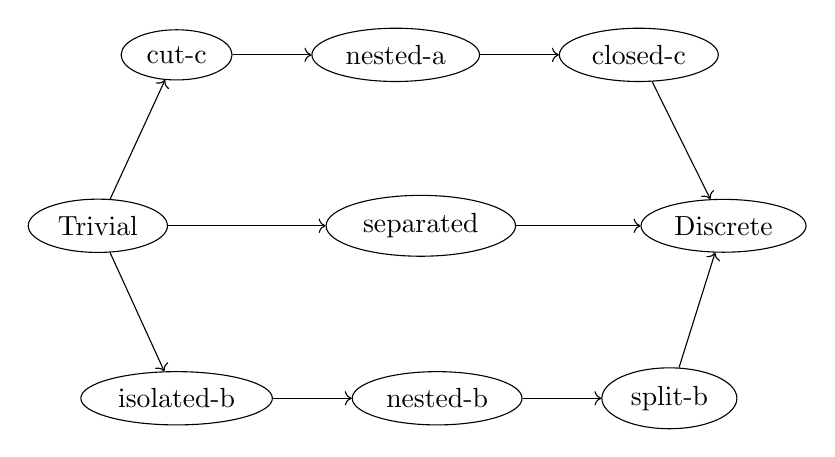
\begin{tikzpicture}[
    node distance=1.5cm and 2cm,
    every node/.style={draw, ellipse, align=center},
    every edge/.style={draw, -{Latex[length=3mm]}}
    ]

    % Nodes
    \node (trivial) {Trivial};
    \node (cutc) [above=of trivial, xshift=1cm] {cut-c};
    \node (nesteda) [above=of cutc, right=of cutc, xshift=-1cm] {nested-a};
    \node (closedc) [right=of nesteda, xshift=-1cm] {closed-c};
    \node (discrete) [right=of trivial, xshift=4cm] {Discrete};

    \node (isolatedb) [below=of trivial, xshift=1cm] {isolated-b};
    \node (nestedb) [right=of isolatedb, xshift=-1cm] {nested-b};
    \node (splitb) [right=of nestedb, xshift=-1cm] {split-b};

    \node (separated) [right=of trivial, xshift=0cm] {separated};

    % Edges
    \draw[->] (trivial) -- (cutc);
    \draw[->] (cutc) -- (nesteda);
    \draw[->] (nesteda) -- (closedc);
    \draw[->] (closedc) -- (discrete);

    \draw[->] (trivial) -- (isolatedb);
    \draw[->] (isolatedb) to (nestedb);
    \draw[->] (nestedb) to (splitb);
    \draw[->] (splitb) -- (discrete);

    \draw[->] (trivial) -- (separated);
    \draw[->] (separated) -- (discrete);

  \end{tikzpicture}
\end{center}
\end{document}

\end{document}
